\section{Description}
Consider the theater ticket reservation system.  You have built this system, 
and now you are responsible for the operation.  Your customer is quite happy 
with the system, except for the availability and, occasionally, the response 
time.  You’ve been in operation for 10 weeks.  To date, the availability of the
system components have been:
\begin{itemize}
    \item \textbf{Hardware} 99.9\%
    \item \textbf{Software}: 99.8\%
    \item \textbf{External Credit card verification and billing system}: 99.0\%
\end{itemize}

The credit card system is required on only 30\% of all transactions, and the 
implementation allows other transactions and the system to work even if the 
credit card system is unavailable.

\pagebreak

\subsection{Calculate the system’s continuous availability percentage.}
The first step is to create a topology that explains how the system is integrated.
\begin{center}
    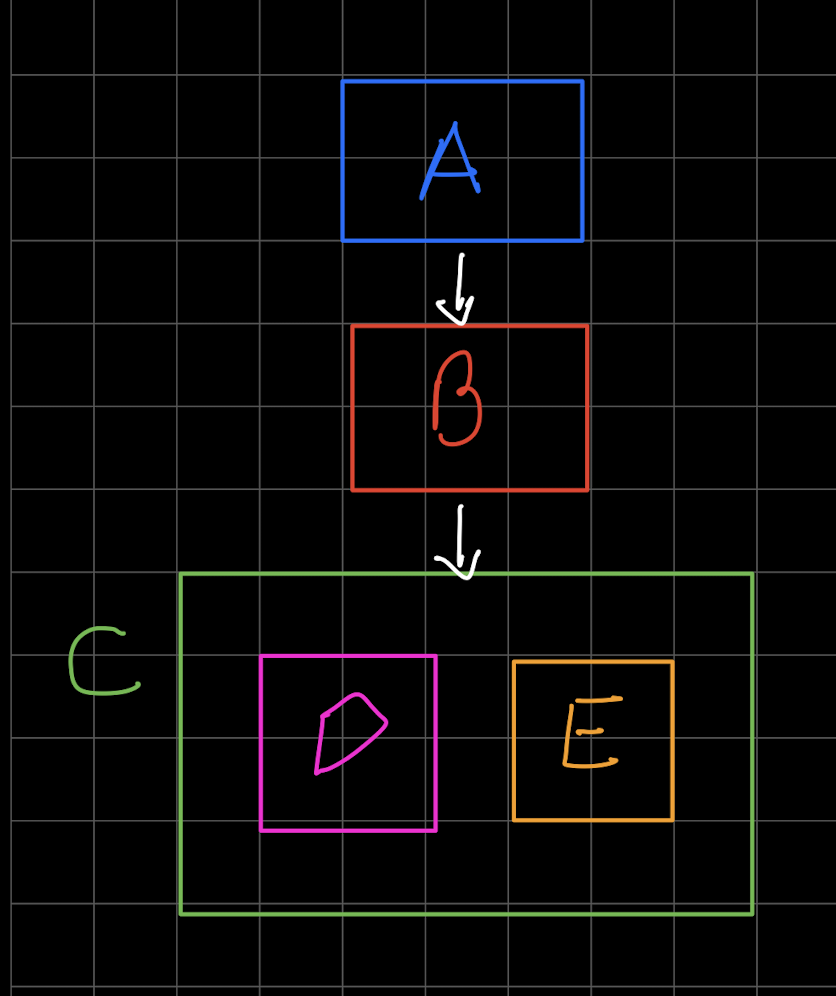
\includegraphics[scale=0.57]{diagram-1.png}    
\end{center}
\noindent
In this diagram we have the Hardware as \textbf{A}, the software as \textbf{B} 
and we introduce a new abstraction that we will call \textit{Payment Module} as 
\textbf{C} know this payment module is going to handle all the transactions, it 
includes the \textbf{External Credit card verification and billing system} as a
submodule which we will call \textbf{D} and an internal billing module called 
\textbf{E}, which we are going to asume that is 100\% available. \newline\newline
\pagebreak

\noindent
\textit{Why did we did this?}\newline\newline
\noindent
Because the description says that 30\% of all transactions 
are credit card transactions which are handled by the component \textbf{D}, that 
means that the 70\% remaining transactions, let say cash, is handle by something 
else, that something else is the submodule \textbf{E}, both of this component 
work together to create the component \textbf{C}.\newline\newline
\noindent
Right now we know the availability of component \textbf{A} and \textbf{B}, but 
we need to calculate the availability of component \textbf{C}.
\[ C = D * 0.3 + E * 0.7 \]
\[ C = (0.99 * 0.3) + (1 * 0.7) \]
\[ C =  0.297 + 0.7 \]
\[ C =  0.997 = 99.7\% \]

\noindent
As we can see from the diagram, module \textbf{A}, \textbf{B} and 
\textbf{C} are in a serial configuration so the continuous availability 
\textbf{CA} would be \textbf{99.4\%}:
\[ CA = A(A) * A(B) * A(C) \]
\[ CA =  99.9\% * 99.8\% * 99.7\%\]
\[ CA =  0.999 * 0.998 * 0.997\]
\[CA = 0.994 = 99.4\%\]

\pagebreak

\subsection{Hot Backup System}
What would be the change in availability if you implement a hot backup system 
to reduce the scheduled maintenance time by 90\%? \newline\newline

\noindent
We know that this change would be applied to the hardware, and we want to reduce 
the maintenance time, not the availability, by 90\%. First we need to know 
what maintenance time is to see how much we are reducing, which 
is \textbf{1680} hours.
\[ Maintenance = 7 * 24 * 10 \]
\[ Maintenance = 1680 hours \]
Since we have a 99.9\% of availability right now, so we have \textbf{0.1\%} of
downtime. 
\[ Downtime = 1680 * 0.1 / 100 = 1.68 hours \]
If we reduce the downtime by 90\%, that means that the 10\% will tells us the 
final amount of downtime that we will have with the hotbackup system which is 
\textbf{0.168} hours.
\[ Downtime = 1.68 * 10 / 100 = 0.168 hours \]
So the new availability for the hardware would be \textbf{99.99\%}: 
\[ A(A) = 100 - (100 * 0.168 / 1680) = 99.99\% \]

\pagebreak

\subsection{Improve the credit card vendor availability}
